\PassOptionsToPackage{unicode=true}{hyperref} % options for packages loaded elsewhere
\PassOptionsToPackage{hyphens}{url}
%
\documentclass[]{article}
\usepackage{lmodern}
\usepackage{amssymb,amsmath}
\usepackage{ifxetex,ifluatex}
\usepackage{fixltx2e} % provides \textsubscript
\ifnum 0\ifxetex 1\fi\ifluatex 1\fi=0 % if pdftex
  \usepackage[T1]{fontenc}
  \usepackage[utf8]{inputenc}
  \usepackage{textcomp} % provides euro and other symbols
\else % if luatex or xelatex
  \usepackage{unicode-math}
  \defaultfontfeatures{Ligatures=TeX,Scale=MatchLowercase}
\fi
% use upquote if available, for straight quotes in verbatim environments
\IfFileExists{upquote.sty}{\usepackage{upquote}}{}
% use microtype if available
\IfFileExists{microtype.sty}{%
\usepackage[]{microtype}
\UseMicrotypeSet[protrusion]{basicmath} % disable protrusion for tt fonts
}{}
\IfFileExists{parskip.sty}{%
\usepackage{parskip}
}{% else
\setlength{\parindent}{0pt}
\setlength{\parskip}{6pt plus 2pt minus 1pt}
}
\usepackage{hyperref}
\hypersetup{
            pdftitle={Relative efficiency of a chain sweep and the rockhopper sweep used for bottom trawl surveys and biomass estimates for flatfish, red hake and goosefish stocks in Northwest Atlantic waters of the United States},
            pdfauthor={Timothy J. Miller1, David E. Richardson2, Andrew Jones2, Phil Politis1},
            pdfborder={0 0 0},
            breaklinks=true}
\urlstyle{same}  % don't use monospace font for urls
\usepackage[margin=1in]{geometry}
\usepackage{graphicx,grffile}
\makeatletter
\def\maxwidth{\ifdim\Gin@nat@width>\linewidth\linewidth\else\Gin@nat@width\fi}
\def\maxheight{\ifdim\Gin@nat@height>\textheight\textheight\else\Gin@nat@height\fi}
\makeatother
% Scale images if necessary, so that they will not overflow the page
% margins by default, and it is still possible to overwrite the defaults
% using explicit options in \includegraphics[width, height, ...]{}
\setkeys{Gin}{width=\maxwidth,height=\maxheight,keepaspectratio}
\setlength{\emergencystretch}{3em}  % prevent overfull lines
\providecommand{\tightlist}{%
  \setlength{\itemsep}{0pt}\setlength{\parskip}{0pt}}
\setcounter{secnumdepth}{5}
% Redefines (sub)paragraphs to behave more like sections
\ifx\paragraph\undefined\else
\let\oldparagraph\paragraph
\renewcommand{\paragraph}[1]{\oldparagraph{#1}\mbox{}}
\fi
\ifx\subparagraph\undefined\else
\let\oldsubparagraph\subparagraph
\renewcommand{\subparagraph}[1]{\oldsubparagraph{#1}\mbox{}}
\fi

% set default figure placement to htbp
\makeatletter
\def\fps@figure{htbp}
\makeatother

\usepackage{url}
\usepackage{setspace}
%\singlespacing
%\onehalfspacing
\doublespacing
\usepackage{lineno}
\linenumbers
\usepackage[belowskip=0pt,aboveskip=0pt]{caption}
\usepackage{relsize}
\usepackage{bm}
\usepackage{caption,graphics}
\usepackage{graphicx}
\renewcommand\figurename{Fig.}
\captionsetup{labelsep=period, singlelinecheck=false}
\usepackage{booktabs}
\usepackage{longtable}
\usepackage{array}
\usepackage{multirow}
\usepackage{wrapfig}
\usepackage{float}
\usepackage{colortbl}
\usepackage{pdflscape}
\usepackage{tabu}
\usepackage{threeparttable}
\usepackage{threeparttablex}
\usepackage[normalem]{ulem}
\usepackage{makecell}
\usepackage{xcolor}

\title{Relative efficiency of a chain sweep and the rockhopper sweep used for
bottom trawl surveys and biomass estimates for flatfish, red hake and
goosefish stocks in Northwest Atlantic waters of the United States}
\author{Timothy J. Miller\textsuperscript{1}, David E.
Richardson\textsuperscript{2}, Andrew Jones\textsuperscript{2}, Phil
Politis\textsuperscript{1}}
\date{}

\begin{document}
\maketitle

\(^1\)\href{mailto:timothy.j.miller@noaa.gov}{\nolinkurl{timothy.j.miller@noaa.gov}},
Northeast Fisheries Science Center, National Marine Fisheries Service,
166 Water Street, Woods Hole, MA 02543, USA\\
\(^2\)Northeast Fisheries Science Center, National Marine Fisheries
Service, Narragansett, RI USA\\

\pagebreak

\hypertarget{abstract}{%
\subsection*{Abstract}\label{abstract}}
\addcontentsline{toc}{subsection}{Abstract}

Using a general hierarchical model we estimated relative efficiency of
chain sweep to the rockhopper sweep used by the NEFSC bottom trawl
survey for from studies carried out between 2015 and 2017 aboard the F/V
Karen Elizabeth twin-trawl vessel. Aside from the sweeps, the rest of
the trawl gear is the same. We compared a set of models with different
assumptions about variation of relative efficiency between paired gear
tows, size and diel effects on the relative efficiency, and
extra-binomial variation of observations within paired gear tows.

Using a general hierarchical model we estimated relative efficiency of
chain sweep to the rockhopper sweep used by the NEFSC bottom trawl
survey for winter and windowpane flounder stocks and red hake stocks
from studies carried out between 2015 and 2017 aboard the F/V Karen
Elizabeth twin-trawl vessel. Aside from the sweeps, the rest of the
trawl gear is the same. We compared a set of models with different
assumptions about variation of relative efficiency between paired gear
tows, size and diel effects on the relative efficiency, and
extra-binomial variation of observations within paired gear tows. Diel
effects provided improved model performance for all three species. We
used the best performing model to make annual chain sweep-based swept
area biomass and abundance-at-length estimates. We estimated uncertainty
in all results using bootstrap procedures for each data component.

\hypertarget{keywords}{%
\subsubsection*{Keywords}\label{keywords}}
\addcontentsline{toc}{subsubsection}{Keywords}

leatherback; habitat; movement; Continuous-time semi-Markov;
environmental effects; GPS tags

\pagebreak

\hypertarget{introduction}{%
\section{Introduction}\label{introduction}}

Paired-gear studies have long been used to estimate the efficiency of
one fishing gear relative to another (e.g., Gulland (1964);Bourne
(1965)). These types of studies are critical for informing abundance
time series from fishery independent surveys when there are changes in
the vessel and(or) gears over time due to gear failures or improved
technology.

In conducting paired-gear studies it is ideal to have the two gears
deployed as close together spatially and temporally as possible to
reduce variation between the gears in densities of the species being
captured. One fishing method that approaches this ideal is the
twin-trawl rigging where two trawls can be fished simultaneously (ICES
1996). The basic methods we used here are based on those used by Miller
(2013) to estimate size effects on relative catch efficiency of the
Henry B. Bigelow to the Albatrosss IV. Similar approaches were used to
make similar estimates for groundfish, TRAC stocks and summer flounder
(Miller et al. 2017a, 2017b). The methods here are the same as those
used for red hake for the red hake research track assessments (Miller et
al. 2020).

\hypertarget{methods}{%
\section{Methods}\label{methods}}

\hypertarget{data-collection}{%
\subsection{Data collection}\label{data-collection}}

Data were collected during three field experiments carried out in 2015,
2016, and 2017, respectively, aboard the F/V Karen Elizabeth, a 78ft
stern trawler capable of towing two trawls simultaneously side by side.
However, red hake were only observed during the 2017 field experiments.
One side of the twin-trawl rig towed a NEFSC standard 400 x 12 cm survey
bottom trawl rigged with the NEFSC standard rockhopper sweep (Politis et
al. 2014) (Figure \ref{rockhopper_schematic}). The other side of the
twin-trawl rig towed a version the NEFSC 400 x 12cm survey bottom trawl
modified to maximize the capture of flatfish. The trawl was modified by
reducing the headline flotation from 66 to 32, 20cm, spherical floats,
reducing the port and starboard top wing-end extensions by 50cm each and
utilizing a chain sweep. The chain sweep was constructed of 1.6cm
(5/8in) trawl chain covered by 12.7cm diameter x 1cm thick rubber discs
on every other chain link (Figure \ref{chainsweep_schematic}). Two rows
of 1.3cm (1/2in) tickler chains were attached to the 1.6cm trawl chain
by 1.3cm shackles (Figure \ref{chainsweep_schematic}). To ensure
equivalent net geometry of each gear, 32m restrictor ropes, made of
1.4cm (9/16in) buoyant, Polytron rope, were attached between each of the
trawl doors and the center clump. 3.4m2 Thyboron Type 4 trawl doors were
used to provide enough spreading force to ensure the restrictor ropes
remained taut throughout each tow. Each trawl used the NEFSC standard
36.6m bridles. All tows followed the NEFSC standard survey towing
protocols of 20 minutes at 3.0 knots. In 2015, 108 (45 day, 63 night)
paired tows were conducted in eastern Georges Bank and off of southern
New England (Figure \ref{2015_tow_locations}). In 2016, 117 (74 day, 43
night) paired tows were conducted in western Gulf of Maine and northern
edge of Georges Bank (Figure \ref{2016_tow_locations}). In 2017, 103 (61
day, 42 night) paired tows were conducted in waters off of southern New
England (Figure \ref{2017_tow_locations}). Paired tows were denoted as
\texttt{day\textquotesingle{}\textquotesingle{}\ and}night'' by whether
the sun was above or below the horizon at the time of the tow.

Winter flounder were caught in 171 paired tows (97 day, 74 night).
Overall 6,449 winter flounder were measured for length. The subsampling
fractions implied an estimated 6,586 winter flounder were captured
across all paired tows. 3805 and 2644 length measurements were made for
the chainsweep and rockhopper gears, respectively. During the day, 2385
and 1220 winter flounder were measured in catches by the respective
gears whereas during the night 1420 and 1424 were measured in catches by
the respective gears.

Windowpane flounder were caught in 195 paired tows (100 day, 95 night).
Overall 13,014 windowpane were measured for length. The subsampling
fractions implied an estimated 15,310 windowpane were captured across
all paired tows. 9854 and 3160 length measurements were made for the
chainsweep and rockhopper gears, respectively. During the day, 5443 and
778 windowpane were measured in catches by the respective gears whereas
during the night 4411 and 2382 were measured in catches by the
respective gears.

Red hake were caught in 73 paired tows (40 day, 33 night). Overall
12,585 red hake were measured for length. The subsampling fractions
implied an estimated 47,275 red hake were captured across all paired
tows. 8587 and 3998 length measurements were made for the chainsweep and
rockhopper gears, respectively. During the day, 4908 and 1706 red hake
were measured in catches by the respective gears whereas during the
night 3679 and 2292 were measured in catches by the respective gears.

\hypertarget{paired-tow-analysis}{%
\subsection{Paired-tow analysis}\label{paired-tow-analysis}}

We use the hierarchical modeling approach from Miller (2013) to estimate
the relative efficiency of chain sweep to the rockhopper sweep used by
the NEFSC bottom trawl survey for six species from three studies carried
out aboard a twin trawl vessel. Aside from the sweeps the rest of the
trawl gear is the same. As in Miller (2013), we compared a set of models
with different assumptions about variation of relative efficiency
between paired gear tows, size effects on the relative efficiency, and
extra-binomial variation of observations within paired gear tows. We
began with the same 13 models considered by Miller (2013). Models
BI\(_1\) to BI\(_4\) and BB\(_1\) to BB\(_8\) in Table
\ref{models_table_winter} provides a descriptions of the models fitted
for all species and pseudo-formulas comparable to those used for fitting
models in R and the mgcv package (Wood 2006; R Core Team 2019). We then
also included diel effects on relative catch efficiency and
intereactions with size effects with the best performing model of the
original 13 models for each species. For red hake, these are the same
analyses provided in Miller et al. (2020) and the new analyses for
winter and windowpane flounder are analogous. The analyses here and in
Miller et al. (2020) are similar to those by Miller et al. (2017a),
Miller et al. (2017b), and Miller et al. (2018), but a more generalized
model has been implemented that allows multiple smooth effects on
relative catch efficiency so that models do not have to be fit
separately to observations occurring during the day and night.
Therefore, diel effects on relative catch efficiency and interactions
with size effects can be considered while allowing other parameters to
be the same for all observations.

\hypertarget{length-weight-analysis}{%
\subsection{Length-weight analysis}\label{length-weight-analysis}}

We fit length-weight relationships to the length and weight observations
for each survey each year. We assumed weight observation \(j\) from
survey \(i\), was log-normal distributed, \begin{equation}\label{wal}
 \log W_{ij} \sim \text{N}\left(\log \alpha_i + \beta_i \log L_{ij} - \frac{\sigma_i^2}{2}, \sigma_i^2\right)
\end{equation} We used a bias correction to ensure the expected weigth
\(E(W_{ij})= \alpha_i L_{ij}^{\beta_i}\). We estimated parameters by
maximizing the model likelihood programmed in TMB (Kristensen et al.
2016) and R (R Core Team 2019). Like the relative catch efficiency,
bootstrap predictions of weight at length were made by sampling with
replacement the length-weight observations within each annual survey and
refitting the length-weight relationship to each of the bootstrap data
sets.

\hypertarget{biomass-estimation}{%
\subsection{Biomass estimation}\label{biomass-estimation}}

We estimated biomass for each annual survey in terms of chainsweep
efficiency by scaling the survey tow observations by the relative
efficiency of the chainsweep and rockhopper sweep gears. First the
tow-specific catches at length are rescaled, \begin{equation}\label{nal}
\widetilde N_{hi}\left(L\right) = N_{hi}\left(L\right)\widehat \rho_i\left(L\right)
\end{equation} where \(N_{hi}(L)\) is the number at length \(L\) in tow
\(i\) from stratum \(h\) and \(\widehat \rho_i\left(L\right)\) is the
relative efficiency of the chain sweep to rockhopper sweep at length
\(L\) estimated from the twin trawl observations, that may depend on the
diel characteristic of tow \(i\) if that factor is in the best model
fitted to the twin-trawl observations. Note that we have omitted any
subscripts denoting the year or survey.

The stratified abundance estimate is then calculated using the
design-based estimator, \begin{equation}\label{Nal_estimate}
 \widehat N(L) = \sum^H_{h=1} \frac{A_h}{An_h}\sum^{n_h}_{i=1} \widetilde N_{hi}(L)
\end{equation} where \(A_h\) is the area of stratum \(h\),
\(A=\sum^H_{h=1} A_h\), and \(n_h\) is the number of tows that were made
in stratum h. The corresponding biomass estimate is then
\begin{equation}\label{biomass_estimate}
 \widehat B = \sum^{n_L}_{l=1} \widehat N(L = l) \widehat w(L=l)
\end{equation} where \(\widehat w(L=l)\) is the estimated weight at
length from fitting length-weight observations described above. Length
is typically measured to the nearest cm so \(n_L\) indicates the number
of 1 cm length categories that were observed during the survey.

To estimate uncertainty in biomass, we used bootstrap results for the
relative catch efficiency and weight at length estimates along with
bootstrap samples of the survey data. Bootstrap data sets for each of
the annual surveys respected the stratified random designs by resampling
with replacement within each stratum (Smith 1997). For each of the 1000
combined bootstraps, survey observations for bootstrap \(b\) were scaled
with the corresponding bootstrap estimates of relative cookie sweep to
rockhopper sweep efficiency and predicted weight at length, using Eqs.
\ref{Nal_estimate} and \ref{biomass_estimate}.

\hypertarget{results}{%
\section{Results}\label{results}}

\hypertarget{winter-flounder}{%
\subsection{Winter flounder}\label{winter-flounder}}

As measured by AIC, the best performing model for winter flounder before
considering day/night effects was the conditional binomial model
BI\(_4\) (Table \ref{models_table_winter}). Allowing smooth size-effects
on relative catch efficiency and variation in these effects among
paired-tows provided primary improvements in model performance.
Including diel effects on relative efficiency for the twin-trawl
observations improved performance of the binomial model (BI\(_5\)),
however the model allowing the size effects on relative efficiency to
differ between day and night (BI\(_6\)) would not converge. The relative
efficiency of the chain sweep gear to the rockhopper sweep gear is
greatest at the smallest sizes of winter flounder, but is fairly
constant over over sizes greater than 25 cm. The minimum relative
efficency is between 1.5 and 2 during the day, but efficiencies of the
two sweeps are approximately equal efficiency at night (Figure
\ref{combined_rhos_winter}).

Stock-specific biomass estimates from 2009 to 2019 for the NEFSC spring
and fall survey were variable. Georges Bank winter flounder biomass
estimates range between 1800 and 9400 mt in the spring and 3000 and
24,000 mt in the fall and are lower in recent years than those in the
early years (Figure \ref{gb_winter_flounder_biomass} and Table
\ref{biomass_table_winter}). However, we note that the estimates of
biomass made here were determined in the 2019 assessment to be
problematic because of the larger sizes that predominate in the Georges
Bank stock area than other stock areas and the low number of
observations in the chainsweep study of these larger individuals (NEFSC
2020). Gulf of Maine winter flounder biomass estimates are constrained
to the segment of the population at least 30 cm in length. The spring
biomass estimates have been fairly stable ranging between 900 and 2700
mt whereas the fall estimates were greater at the beginning of the time
series than recent years and range between 1900 and 4300 mt (Figure
\ref{gom_winter_flounder_biomass} and Table \ref{biomass_table_winter}).
Southern New England winter flounder biomass estimates are also lower in
recent years than the beginning of the time series for both seasons and
spring and fall estimates range from 1300 to 8500 mt and 2100 to 47,500
mt, respectively (Figure \ref{sne_winter_flounder_biomass} and Table
\ref{biomass_table_winter}).

The efficiency of the rockhopper gear relative to the chainsweep in
terms of biomass changes from year to year due primarily to
corresponding changes in the estimated numbers at length (Table
\ref{biomass_efficiencies_winter}). Annual biomass relative efficiency
for Georges Bank winter flounder varied between 0.55 and 0.79 in the
spring and 0.61 and 0.92 in the fall. Relative efficiencies for the Gulf
of Maine stock range between 0.54 and 0.70 for the spring and 0.63 and
0.88 in the fall. Relative efficiencies for the Southern New England
stock range between 0.64 and 0.91 for the spring and 0.60 and 1.0 for
the fall.

Because the length-weight relationship which is used with the numbers at
length to estimate biomass is estimated by survey and year there is a
possibility that poor sampling in a given year could adversely affect
the biomass estimates. We therefore calculated the ratios of the annual
uncalibrated biomass estimates using just the aggregate catch data to
the biomass estimates made using the numbers at length and estimated
weight at length (i.e., Eqs. \ref{Nal_estimate} and
\ref{biomass_estimate} without the relative efficiency at size). These
ratios should be approximately 1. The ratios for all years and seasons
for all three stocks of winter flounder varied from 0.94 to 1.04 (Table
\ref{biomass_ratios_winter}).

\hypertarget{windowpane-flounder}{%
\subsection{Windowpane flounder}\label{windowpane-flounder}}

As measured by AIC, the best performing model for windowpane flounder
before considering day/night effects was the conditional binomial model
BI\(_4\) (Table \ref{models_table_windowpane}). Allowing smooth
size-effects on relative catch efficiency and variation in these effects
among paired-tows provided primary improvements in model performance.
Including diel effects on relative efficiency at size for the twin-trawl
observations improved performance of the binomial model (BI\(_6\)). The
relative efficiency of the chain sweep gear to the rockhopper sweep gear
decreases with size of windowpane flounder. The minimum relative
efficiency is between 4.5 and 21 during the day, and between 1.8 and 2.9
at night (Figure \ref{combined_rhos_windowpane}).

Stock-specific biomass estimates from 2009 to 2019 for the NEFSC spring
and fall survey were variable. Georges Bank-Gulf of Maine windowpane
flounder biomass estimates range between 3000 and 20,300 mt in the
spring and 4700 and 18,300 mt in the fall and are lower in recent years
than those in the early years (Figure \ref{gbgom_windowpane_biomass} and
Table \ref{biomass_table_windowpane}). Southern New England-Mid-Atlantic
Bight windowpane flounder biomass estimates in the spring ranged between
7300 and 15,600 mt whereas the fall estimates ranged between 7300 and
14,700 mt (Figure \ref{snemab_windowpane_biomass} and Table
\ref{biomass_table_windowpane}).

The efficiency of the rockhopper gear relative to the chainsweep in
terms of biomass changes from year to year due primarily to
corresponding changes in the estimated numbers at length (Table
\ref{biomass_efficiencies_windowpane}). Annual biomass relative
efficiency for Georges Bank-Gulf of Maine windowpane flounder varied
between 0.21 and 0.36 in the spring and 0.19 and 0.42 in the fall.
Relative efficiencies for the Southern New England-Mid-Atlantic Bight
stock ranged between 0.22 and 0.36 for the spring and 0.26 and 0.35 in
the fall.

Because the length-weight relationship which is used with the numbers at
length to estimate biomass is estimated by survey and year there is a
possibility that poor sampling in a given year could adversely affect
the biomass estimates. We therefore calculated the ratios of the annual
uncalibrated biomass estimates using just the aggregate catch data to
the biomass estimates made using the numbers at length and estimated
weight at length (i.e., Eqs. \ref{Nal_estimate} and
\ref{biomass_estimate} without the relative efficiency at size). These
ratios should be approximately 1. The ratios for all years and seasons
for both stocks of windowpane flounder varied from 0.97 to 1.04 (Table
\ref{biomass_ratios_windowpane}).

\hypertarget{red-hake}{%
\subsection{Red hake}\label{red-hake}}

For red hake, the best performing model before considering day/night
effects was the conditional beta-binomial model BB\(_6\) (Table
\ref{models_table_redhake}). The best beta-binomial model had an AIC
more than 13 units lower than the best binomial model. Allowing
variation in smooth size-effects on relative catch efficiency among
paired-tows and extra-binomial variation withing paired-tows
(overdispersion via the beta-binomial assumption) provided primary
improvements in model performance. Including diel effects on relative
efficiency for the twin-trawl observations improved performance of the
beta-binomial model. Initially separate smooth size effects for day and
night tows were considered for the beta-binomial model (BB\(_8\)), but
the correlation of non-smoother related random effects across stations
was not estimable. Those random effects were therefore assumed
uncorrelated (BB\(_9\)). Allowing different smooth size effects of
relative efficiency for day and night observations was considerd
(BB\(_{10}\)), but it did not improve model performance. The relative
efficiency of the chain sweep gear to the rockhopper sweep gear
generally declines with increased size whether the tow occurred during
day or night, but the increase in efficiency of the chainsweep was
generally greater for tows occuring during the day (Figure
\ref{combined_rhos_redhake}).

Stock-specific trends in annual biomass estimates from 2009 to 2019 for
the NEFSC spring and fall survey were generally the same. For northern
red hake both the spring and fall biomass estimates increased in 2014
and have remained higher than previous years (Figure
\ref{north_red_hake_biomass} and Table \ref{biomass_table_redhake}). The
scale of the biomass estimates is also similar for the spring and fall
surveys. For southern red hake, the spring biomass generally declined
until 2017 and then has increased for the last two years whereas the
fall biomass has remained relatively stable (Figure
\ref{south_red_hake_biomass} and Table \ref{biomass_table_redhake}).

The efficiency of the rockhopper gear relative to the chainsweep in
terms of biomass changes from year to year due primarily to
corresponding changes in the estimated numbers at length (Table
\ref{biomass_efficiencies_redhake}). Annual biomass relative efficiency
for northern red hake varied between 0.19 and 0.25 in the spring and
0.21 and 0.33 in the fall. Values range between 0.15 and 0.26 for the
spring and 0.19 and 0.39 in the fall for southern red hake.

Because the length-weight relationship which is used with the numbers at
length to estimate biomass is estimated by survey and year there is a
possibility that poor sampling in a given year could adversely affect
the biomass estimates. We therefore calculated the ratios of the annual
uncalibrated biomass estimates using just the aggregate catch data to
the biomass estimates made using the numbers at length and estimated
weight at length (i.e., Eqs. \ref{Nal_estimate} and
\ref{biomass_estimate} without the relative efficiency at size). These
ratios should be approximately 1. The ratios for all years and seasons
for both northern and southern red hake varied from 0.96 to 1.04 (Table
\ref{biomass_ratios_redhake}).

\hypertarget{discussion}{%
\section{Discussion}\label{discussion}}

\hypertarget{acknowledgements}{%
\section*{Acknowledgements}\label{acknowledgements}}
\addcontentsline{toc}{section}{Acknowledgements}

\pagebreak

\hypertarget{references}{%
\subsection*{References}\label{references}}
\addcontentsline{toc}{subsection}{References}

\hypertarget{refs}{}
\leavevmode\hypertarget{ref-bourne65}{}%
Bourne, N. 1965. A comparison of catches by 3- and 4-inch rings on
offshore scallop drags. \textbf{22}(2): 313--333.

\leavevmode\hypertarget{ref-gulland64}{}%
Gulland, J.A. 1964. Variations in selection factors, and mesh
differentials. \textbf{29}(2): 158--165.

\leavevmode\hypertarget{ref-ices96}{}%
ICES. 1996. Manual of methods of measuring the selectivity of towed
fishing gears. (Eds.) Wileman, D. A., Ferro, R. S. T., Fonteyne, R., and
Millar, R. B. ICES Cooperative Research Report No. 215.

\leavevmode\hypertarget{ref-kristensenetal16}{}%
Kristensen, K., Nielsen, A., Berg, C.W., Skaug, H., and Bell, B.M. 2016.
TMB: Automatic differentiation and Laplace approximation. Journal of
Statistical Software \textbf{70}(5): 1--21.

\leavevmode\hypertarget{ref-miller13}{}%
Miller, T.J. 2013. A comparison of hierarchical models for relative
catch efficiency based on paired-gear data for U.S. Northwest Atlantic
fish stocks. \textbf{70}(9): 1306--1316.

\leavevmode\hypertarget{ref-milleretal17a}{}%
Miller, T.J., Martin, M., Politis, P., Legault, C.M., and Blaylock, J.
2017a. Some statistical approaches to combine paired observations of
chain sweep and rockhopper gear and catches from NEFSC and DFO trawl
surveys in estimating Georges Bank yellowtail flounder biomass. TRAC
Working Paper 2017/XX. 36p,

\leavevmode\hypertarget{ref-milleretal18}{}%
Miller, T.J., Politis, P., Blaylock, J., Richardson, D., Manderson, J.,
and Roebuck, C. 2018. Relative efficiency of a chain sweep and the
rockhopper sweep used for the NEFSC bottom trawl survey and
chainsweep-based swept area biomass estimates for 11 flatfish stocks.
SAW 66 summer flounder Data/Model/Biological Reference Point meeting.
National Marine Fisheries Service, Northeast Fisheries Science Center,
Woods Hole, MA. September 17-21, 2018.

\leavevmode\hypertarget{ref-milleretal17b}{}%
Miller, T.J., Richardson, D.E., Politis, P., and Blaylock, J. 2017b.
NEFSC bottom trawl catch efficiency and biomass estimates for 2009-2017
for 8 flatfish stocks included in the 2017 Northeast Groundfish
Operational Assessments. 2017 Groundfish Operational Assessment working
paper. Northeast Fisheries Science Center.

\leavevmode\hypertarget{ref-milleretal20}{}%
Miller, T.J., Richardson, D., Politis, P., Blaylock, J., Manderson, J.,
and Roebuck, C. 2020. SAW 66 summer flounder Data/Model/Biological
Reference Point meeting. National Marine Fisheries Service, Northeast
Fisheries Science Center, Woods Hole, MA. September 17-21, 2018.

\leavevmode\hypertarget{ref-nefsc2020}{}%
NEFSC. 2020. Operational assessment of 14 northeast groundfish stocks,
updated through 2018. Prepublication Copy of the September 2019
Operational Stock Assessment Report. The report is ``in preparation''
for publication by the NEFSC. (Oct. 3, 2019; latest revision: Jan. 7,
2020).
https://nefsc.noaa.gov/saw/2019-groundfish-docs/Prepublication-NE-Grndfsh-1-7-2020.pdf.

\leavevmode\hypertarget{ref-politisetal14}{}%
Politis, P.J., Galbraith, J.K., Kostovick, P., and Brown, R.W. 2014.
Northeast Fisheries Science Center bottom trawl survey protocols for the
NOAA Ship Henry B. Bigelow. U.S. Dept. Commer., Northeast Fish. Sci.
Cent. Ref. Doc. 14-06, 138p.

\leavevmode\hypertarget{ref-R19}{}%
R Core Team. 2019. R: A language and environment for statistical
computing. R Foundation for Statistical Computing, Vienna, Austria.
Available from \url{https://www.R-project.org}.

\leavevmode\hypertarget{ref-smith97}{}%
Smith, S.J. 1997. Bootstrap confidence limits for groundfish trawl
survey estimates of mean abundance. \textbf{54}(3): 616--630.

\leavevmode\hypertarget{ref-wood06}{}%
Wood, S.N. 2006. Generalized additive models: An introduction with r.
Chapman \& Hall, Boca Raton, Florida.

\pagebreak

\begin{figure}
\caption{Diagram of the standard Northeast Fisheries Science Center rockhopper sweep center and wing sections.}\label{rockhopper_schematic}
\begin{center}
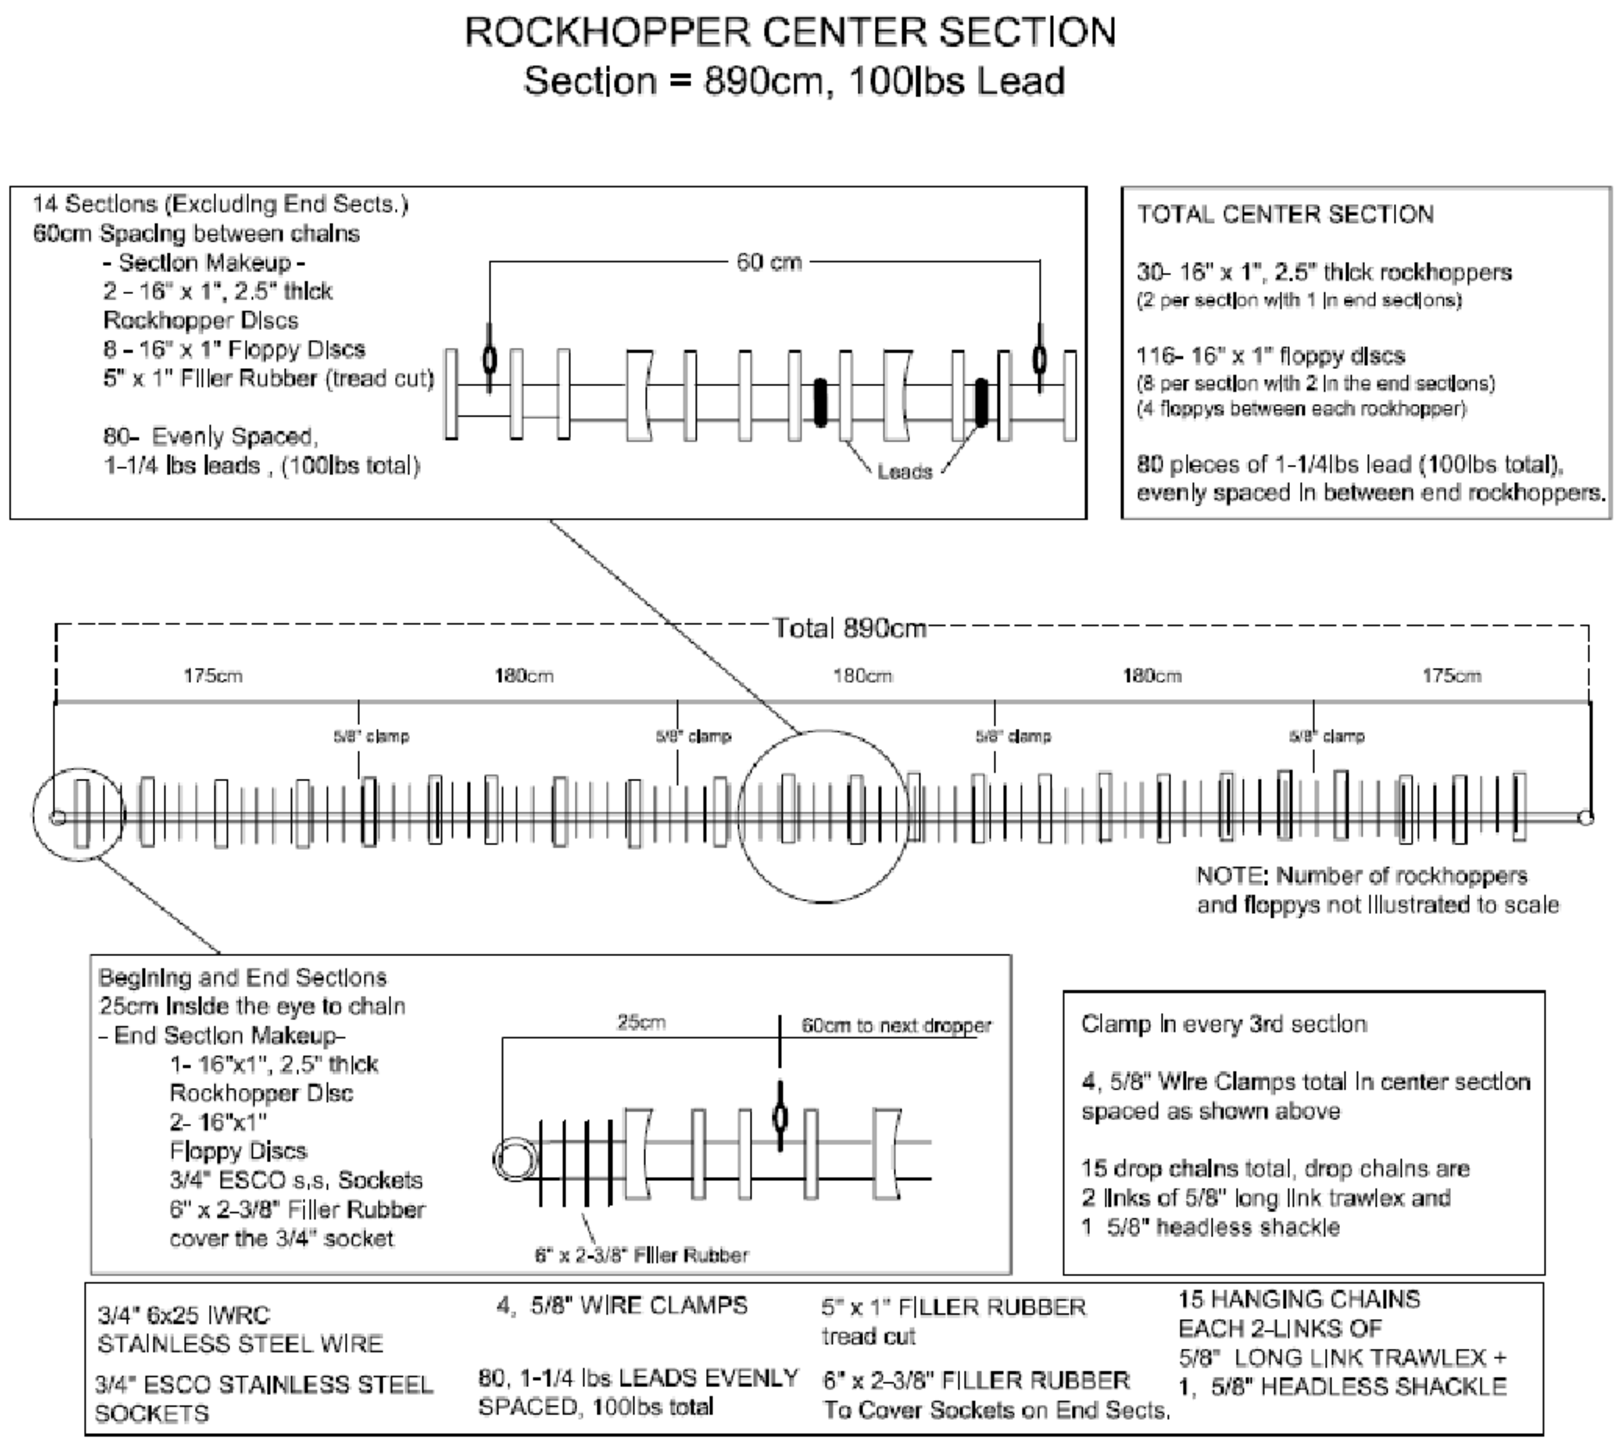
\includegraphics[width = 0.7\textwidth]{rockhopper_schematic_1.pdf}
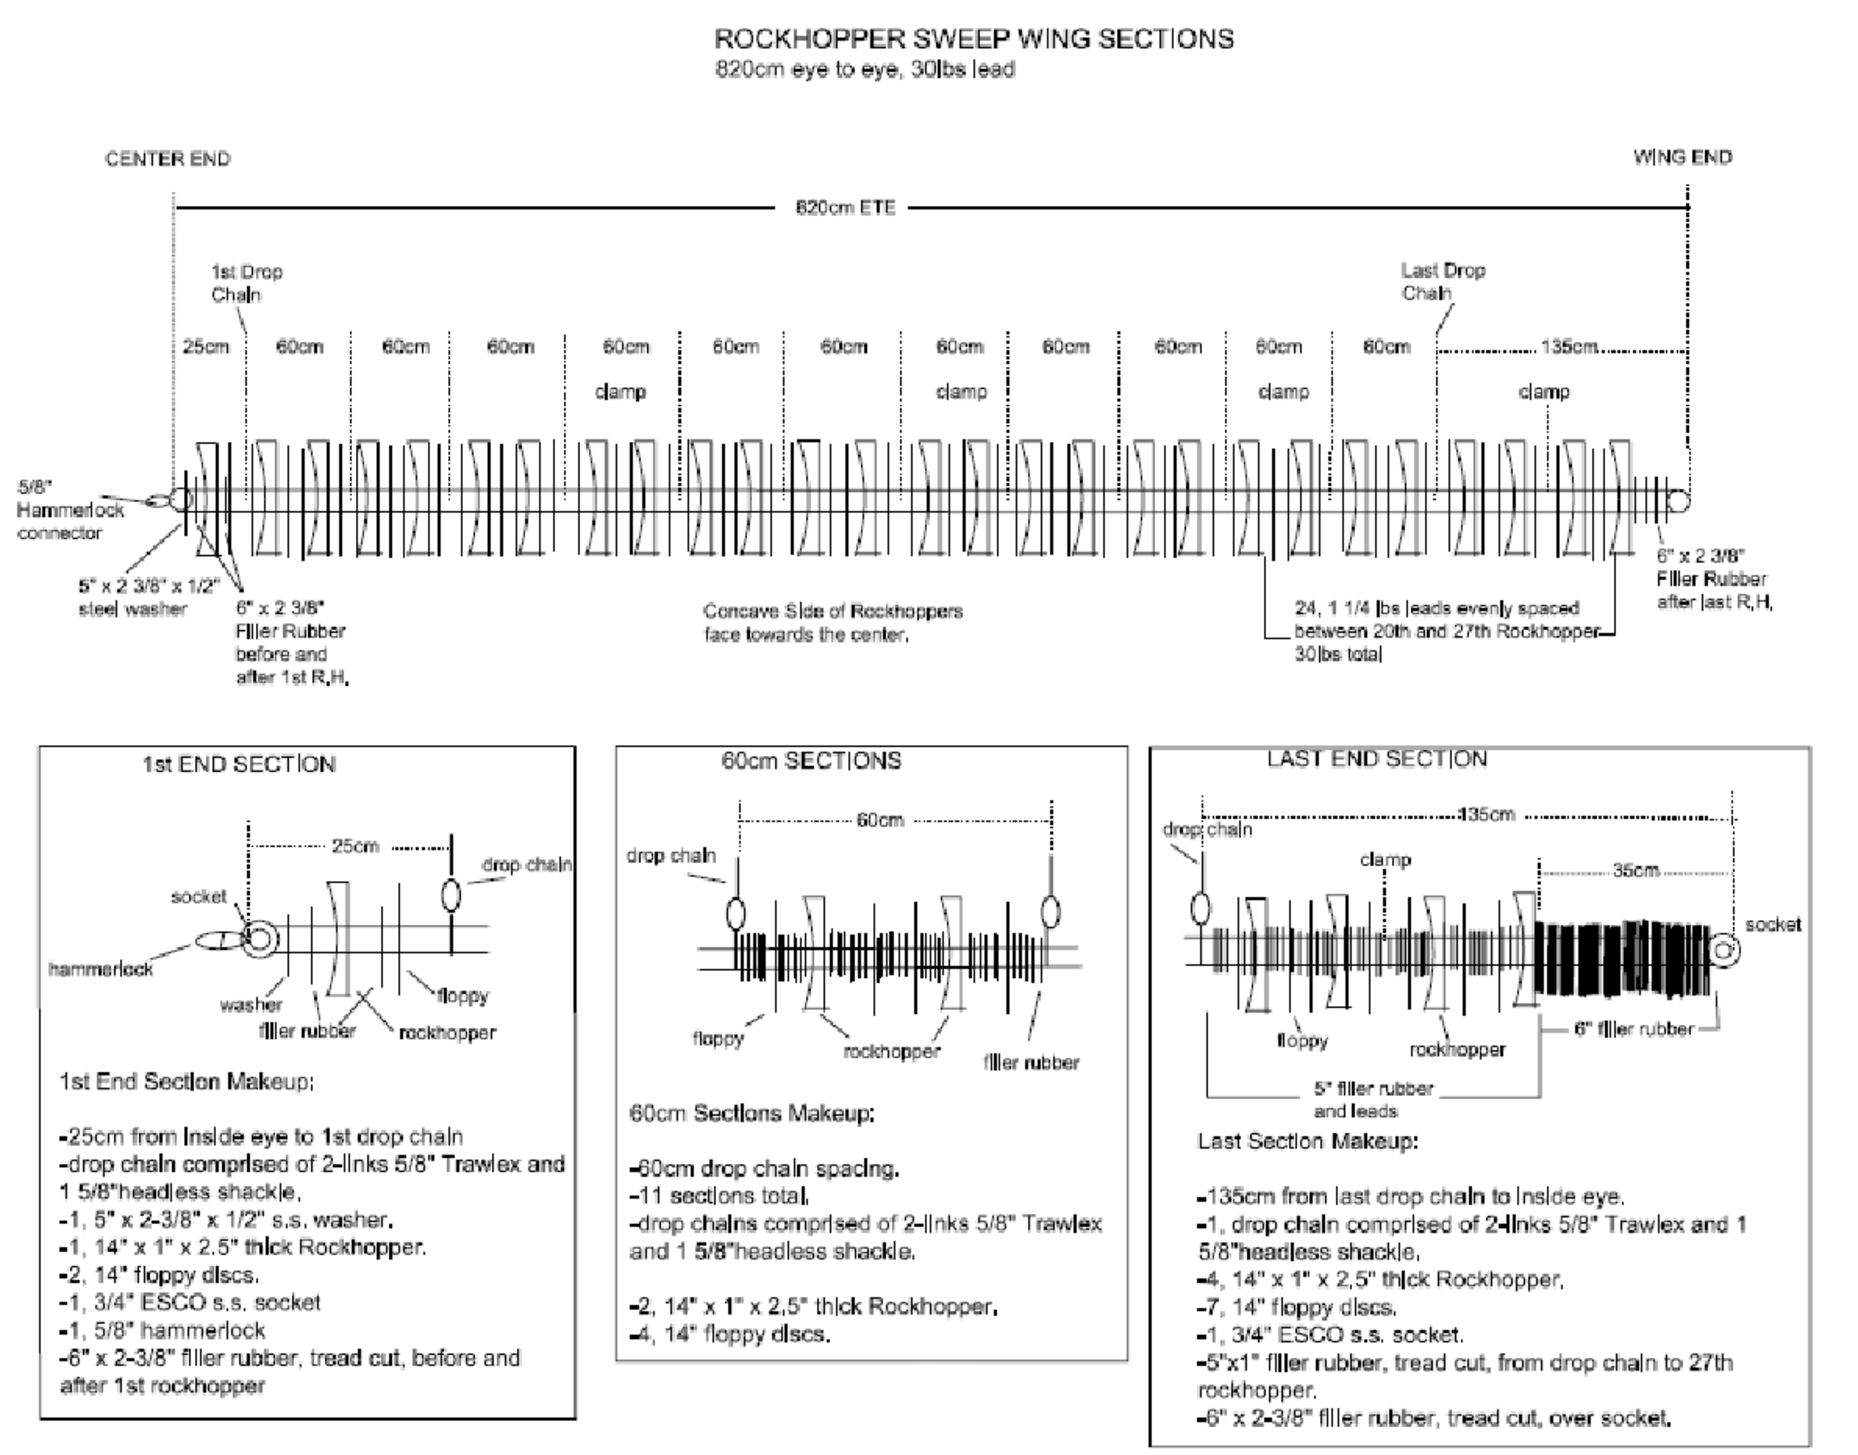
\includegraphics[width = 0.7\textwidth]{rockhopper_schematic_2.pdf}
\end{center}
\end{figure}

\begin{figure}
\caption{Diagram of the chain sweep designed maximize bottom contact and flatfish capture.}\label{chainsweep_schematic}
\begin{center}
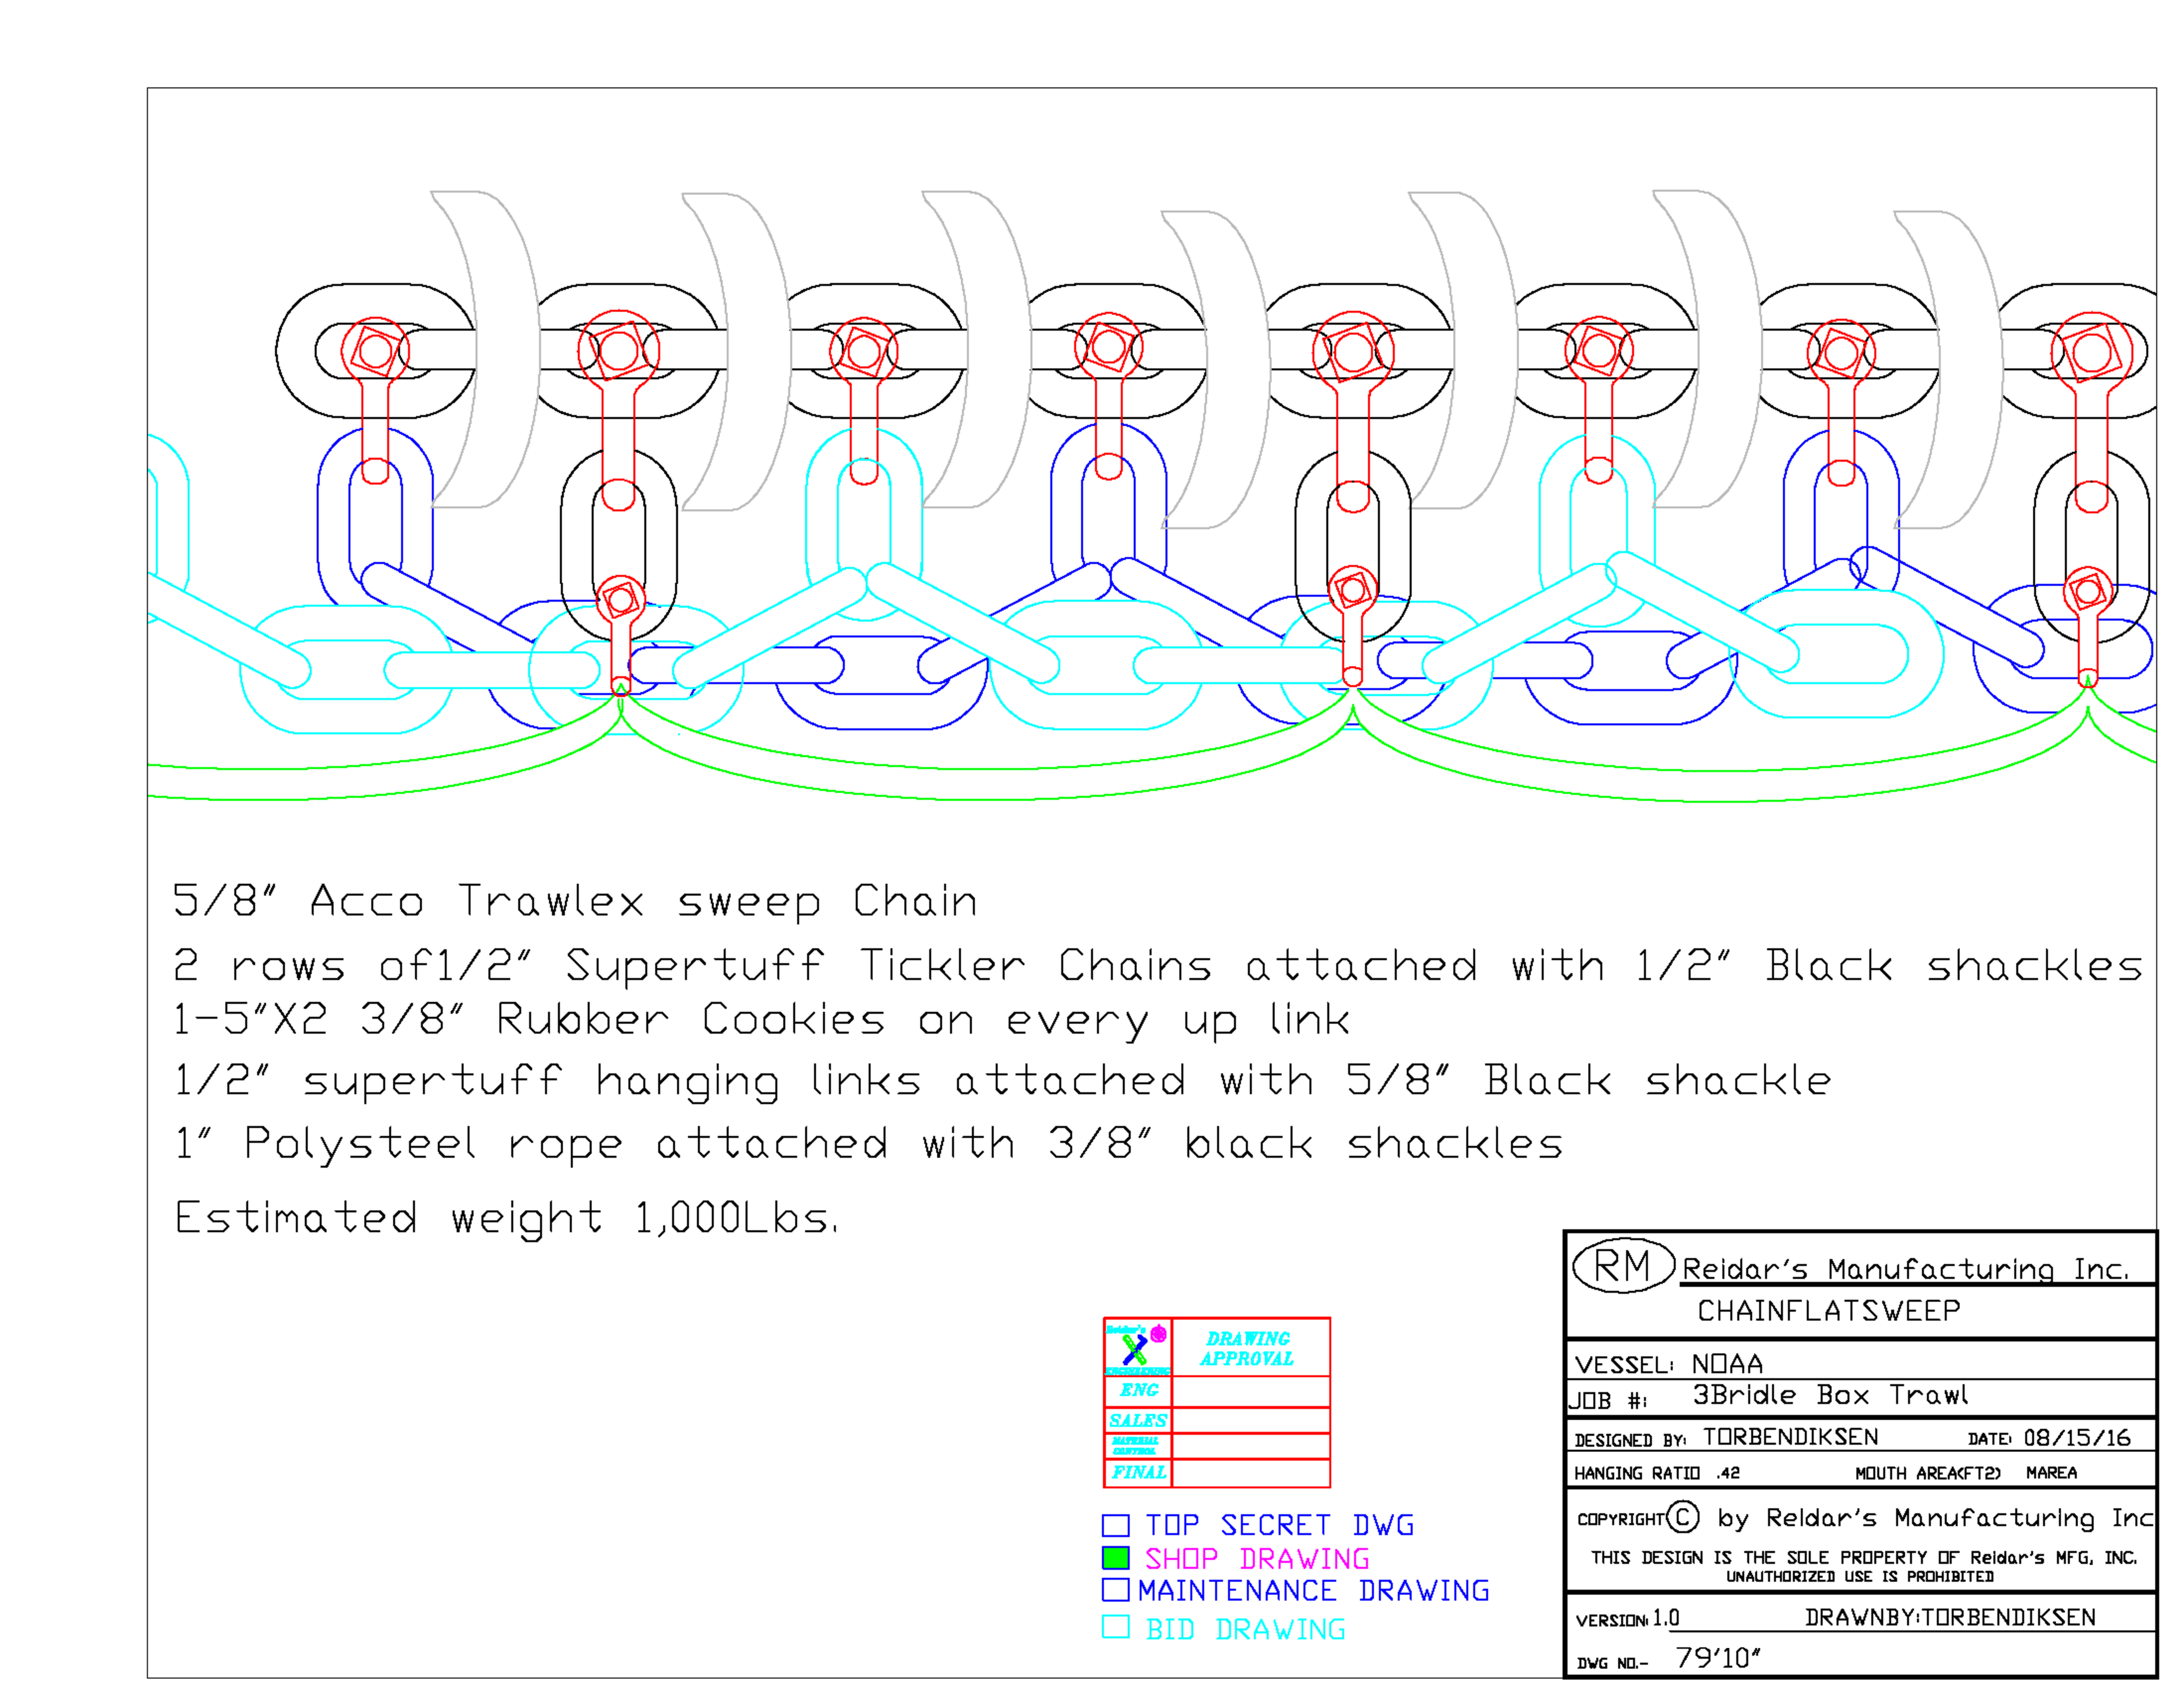
\includegraphics[width = \textwidth]{chainsweep_schematic.pdf}
\end{center}
\end{figure}
\clearpage

\begin{figure}
\caption{Locations of stations in 2015 where the F/V Karen Elizabeth conducted twin-trawl sets with the standard bottom trawl gear and the gear with a chain sweep instead of the rockhopper sweep.}\label{2015_tow_locations}
\begin{center}
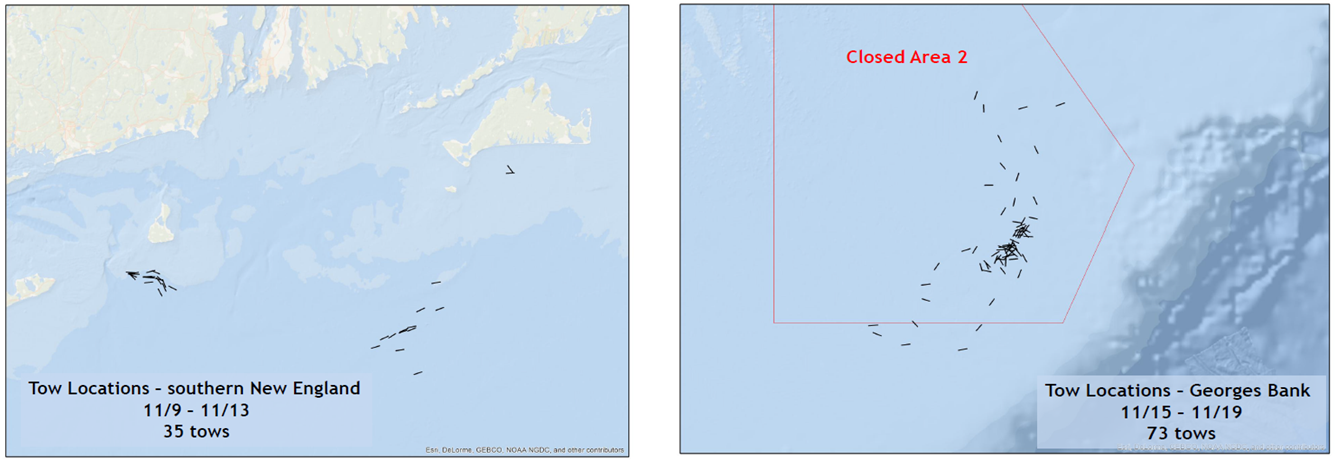
\includegraphics[width = \textwidth]{2015_tow_locations.png}
\end{center}
\end{figure}

\begin{figure}
\caption{Locations of stations in 2016 where the F/V Karen Elizabeth conducted twin-trawl sets with the standard bottom trawl gear and the gear with a chain sweep instead of the rockhopper sweep.}\label{2016_tow_locations}
\begin{center}
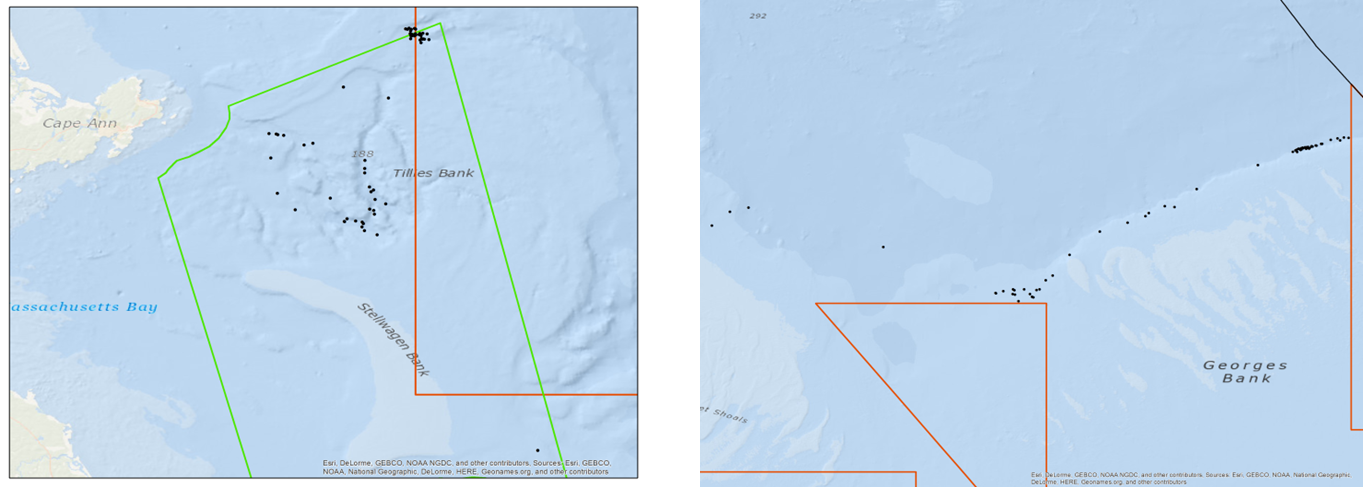
\includegraphics[width = \textwidth]{2016_tow_locations.png}
\end{center}
\end{figure}

\begin{figure}
\caption{Locations of stations in 2017 where the F/V Karen Elizabeth conducted twin-trawl sets with the standard bottom trawl gear and the gear with a chain sweep instead of the rockhopper sweep.}\label{2017_tow_locations}
\begin{center}
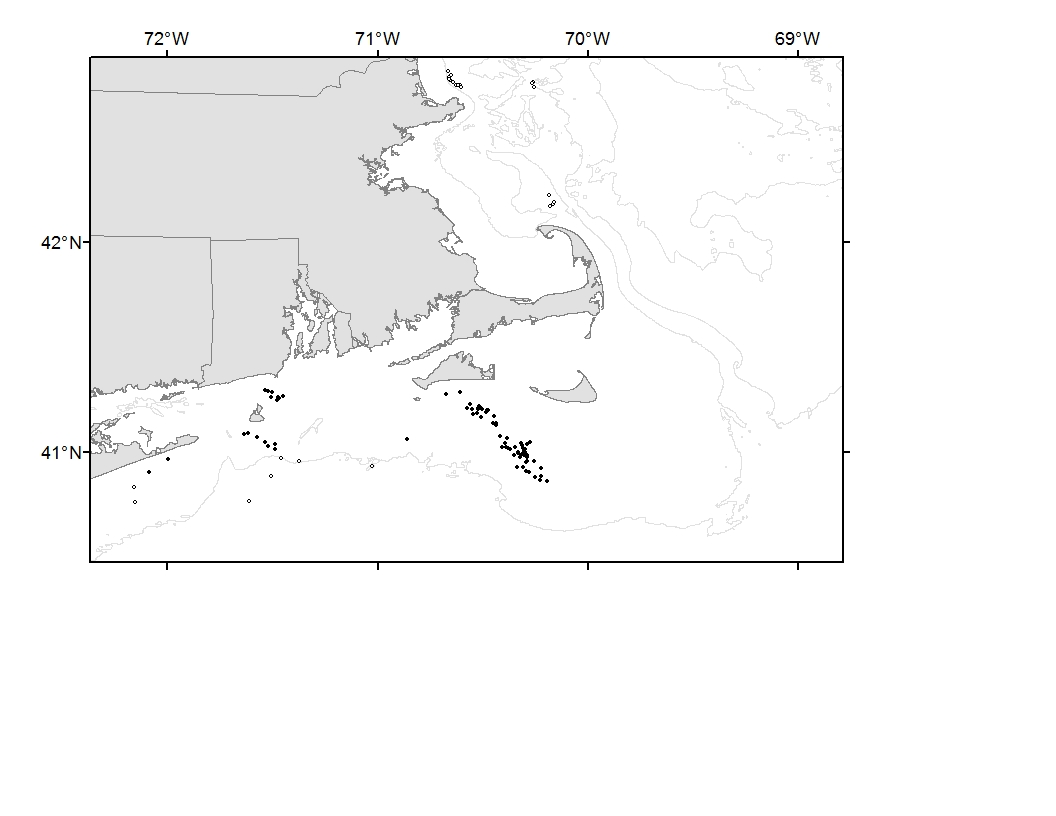
\includegraphics[width = \textwidth]{2017_tow_locations.png}
\end{center}
\end{figure}

\end{document}
